
\begin{figure}
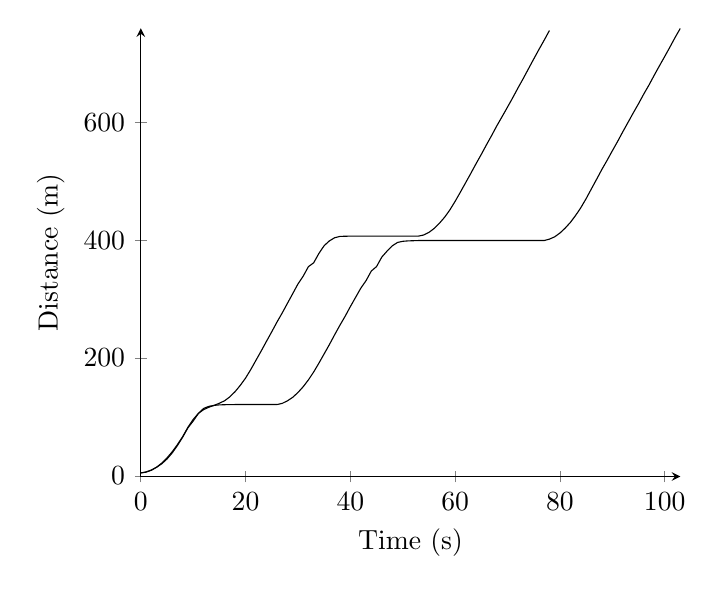
\begin{tikzpicture}
\begin{axis}[
legend style={anchor=west},
axis x line=bottom,
axis y line=left,
ymin=-1,
xlabel=Time (s),
ylabel=Distance (m),
]
\addplot[] coordinates {
(0, 5.1)
(1, 6.79198347547)
(2, 10.0246029611)
(3, 14.5682784754)
(4, 20.5831655964)
(5, 28.6822336373)
(6, 39.0388067366)
(7, 51.6299759322)
(8, 65.792207698)
(9, 81.6290542971)
(10, 93.0743580956)
(11, 105.931037529)
(12, 114.548385896)
(13, 118.041433424)
(14, 119.683803466)
(15, 120.531293121)
(16, 120.817295658)
(17, 121.024355939)
(18, 121.099098764)
(19, 121.110955913)
(20, 121.110955913)
(21, 121.110955913)
(22, 121.110955913)
(23, 121.110955913)
(24, 121.110955913)
(25, 121.110955913)
(26, 121.110955913)
(27, 123.067205587)
(28, 127.498655045)
(29, 133.33109492)
(30, 141.545444916)
(31, 151.292276357)
(32, 162.963714513)
(33, 176.297201366)
(34, 191.333928215)
(35, 207.005379036)
(36, 222.789743613)
(37, 239.385066244)
(38, 255.447089362)
(39, 270.718065541)
(40, 287.170808171)
(41, 302.802524693)
(42, 318.496906084)
(43, 331.267223171)
(44, 347.520941302)
(45, 355.072239431)
(46, 371.131765201)
(47, 381.239886116)
(48, 390.211375458)
(49, 396.008347934)
(50, 397.936406159)
(51, 398.663730609)
(52, 398.961883549)
(53, 399.253715489)
(54, 399.271121774)
(55, 399.271121774)
(56, 399.271121774)
(57, 399.271121774)
(58, 399.271121774)
(59, 399.271121774)
(60, 399.271121774)
(61, 399.271121774)
(62, 399.271121774)
(63, 399.271121774)
(64, 399.271121774)
(65, 399.271121774)
(66, 399.271121774)
(67, 399.271121774)
(68, 399.271121774)
(69, 399.271121774)
(70, 399.271121774)
(71, 399.271121774)
(72, 399.271121774)
(73, 399.271121774)
(74, 399.271121774)
(75, 399.271121774)
(76, 399.271121774)
(77, 399.271121774)
(78, 401.647122674)
(79, 405.563591959)
(80, 411.956118207)
(81, 420.275363604)
(82, 430.021537829)
(83, 441.873190037)
(84, 455.09394477)
(85, 470.245636948)
(86, 486.752955651)
(87, 503.092813246)
(88, 519.686170392)
(89, 535.193059932)
(90, 551.348863897)
(91, 567.098828959)
(92, 583.663961743)
(93, 599.644619707)
(94, 615.719197597)
(95, 631.256359134)
(96, 647.628213023)
(97, 662.989232004)
(98, 679.586174078)
(99, 695.655595717)
(100, 711.345797375)
(101, 727.403861222)
(102, 743.946870337)
(103, 759.344779492)
};
\addplot[] coordinates {
(0, 5.1)
(1, 6.41519215909)
(2, 9.58313743778)
(3, 14.7536180467)
(4, 21.7314005954)
(5, 30.5175190881)
(6, 41.0177092926)
(7, 53.1865627108)
(8, 66.6947371194)
(9, 82.5045063081)
(10, 95.7909209406)
(11, 106.11815493)
(12, 112.506765585)
(13, 116.561993297)
(14, 119.651191916)
(15, 123.325463682)
(16, 127.53542098)
(17, 134.199741365)
(18, 142.963350827)
(19, 153.705194516)
(20, 165.969114041)
(21, 180.501247866)
(22, 196.393663301)
(23, 212.163231922)
(24, 228.449582412)
(25, 244.516049129)
(26, 261.025843367)
(27, 276.483317795)
(28, 292.867125116)
(29, 309.140903051)
(30, 325.56911395)
(31, 338.878846579)
(32, 354.977991153)
(33, 361.475880945)
(34, 377.413770829)
(35, 390.513215033)
(36, 398.671519298)
(37, 403.947845679)
(38, 406.253490683)
(39, 406.5613213)
(40, 406.709109213)
(41, 406.739426242)
(42, 406.739426242)
(43, 406.739426242)
(44, 406.739426242)
(45, 406.739426242)
(46, 406.739426242)
(47, 406.739426242)
(48, 406.739426242)
(49, 406.739426242)
(50, 406.739426242)
(51, 406.739426242)
(52, 406.739426242)
(53, 406.739426242)
(54, 408.672616804)
(55, 413.068780969)
(56, 419.787433352)
(57, 428.525873819)
(58, 438.862134987)
(59, 451.236130882)
(60, 465.751904674)
(61, 481.295881972)
(62, 497.256927953)
(63, 513.240740518)
(64, 529.642540615)
(65, 545.428466948)
(66, 561.929217644)
(67, 577.904474625)
(68, 594.48220008)
(69, 609.93531142)
(70, 625.623582134)
(71, 641.533803549)
(72, 658.082420807)
(73, 674.006858245)
(74, 690.588159066)
(75, 707.09004329)
(76, 723.333889735)
(77, 739.130387251)
(78, 755.471499359)
};

\end{axis}
\end{tikzpicture}
\label{tik:distance:0:107}
\caption{0 percent diving with GSC on route $107$}
\end{figure}
